\documentclass[12p,a4paper]{article}
\usepackage[utf8]{inputenc}
\usepackage[T1]{fontenc,url}
\usepackage{parskip}
\usepackage{lmodern}
\usepackage{microtype}
\usepackage{verbatim}
\usepackage{amsmath, amssymb}
\usepackage{tikz}
\usepackage{physics}
\usepackage{mathtools}
\usepackage{algorithm}
\usepackage{algpseudocode}
\usepackage{listings}
\usepackage{enumerate}
\usepackage{graphicx}
\usepackage{float}
\usepackage{epigraph}
\usepackage{hyperref}
\usepackage{tikz}
\usepackage[a4paper]{geometry}
\begin{document}


\newcommand{\half}{\frac{1}{2}}
\renewcommand{\exp}[1]{\mathrm{e}^{#1}}
\renewcommand{\i}{\mathrm{i}}
\newcommand{\R}{\mathbb{R}}

\newgeometry{left = 0cm, bottom = 0cm, top = 0cm, right = 0cm}

\begin{tikzpicture}[]
\node at (0,0) {
\includegraphics[width=\textwidth]{../oblig_forside_2017.pdf}};
\node[right] at (-7,5.7) {\begin{huge} Jonas Gahr Sturtzel Lunde \end{huge}};
\node[right] at (-6.3,3.77) {\begin{huge} 3 \end{huge}};
\node[right] at (-5.4,1.85) {\begin{huge} 13.02.2017 \end{huge}};
\draw(-0.35,-0.05) circle[radius = 0.5cm];
\end{tikzpicture}

\pagebreak
\restoregeometry 

\section*{Oppgave 1}
Begge metodene for numerisk løsning av differensialligninger baserer seg på å estimere en ukjent funksjon $y(x)$ over et intervall $x, \ x + \Delta x$, gjennom funksjonens kjente derivert, $y'(x)$. Forskjellen er at Eulers metode kun bruker deriverte i starten av intervallet, og ikke tar hensyn til at den deriverte kan endre seg i løpet av intervallet. Runge Kutta metodene bruker derimot en vektet kombinasjon av de deriverte i intervallet $x, \ x + \Delta x$. Dette gir et betydelig bedre estimat for den faktisk løsningen av $y(x)$. Runge Kutta 4 bruker 4 slike vektede deriverte.


\section*{Oppgave 2}
Vi ser at det første pendelet foretar en dempet, tilnærmet harmonisk svingning. Vi vet at utslaget til pendeler kan modeleres som harmoniske svingninger for lave vinkler. Vi merker oss også at utslaget blir mindre over tid, grunnet friksjonen. Fra fasediagramet ser vi at pendelet starter i toppen, med $0\mathrm{rad}$ utslag, og $6 \mathrm{rad/s}$ hastighet. Heretter går denne hastigheten over i en posisjonsforandring, og dette oscileres frem og tilbake, og gir disse sirkelkurvene. Grunnen til at sirklene er mindre er fordi den totale hastigheten og det totale utslaget blir mindre for hver svingning.

Det andre pendelet starter ut på tilsvarende måte, men når det kommer til et utslag $\pi \mathrm{rad}$, som er rett opp, begynner hastigheten å øke. Dette er fordi pendelet har tippet over toppunktet, og fortsetter på en ny runde. Ved et utslag $3\pi\mathrm{rad}$, som representerer toppen på en ny runde, ser vi at pendelen står stille et øyeblikk, før det faller tilbake der det kom fra, og ikke tar en ny runde. På grunn av friksjonen er ikke lenger den kinetiske energien stor nok til å frakte pendelet over toppen, og vi ser at kurven nå får en tilsvarende form som for det forrige pendelet. Svingningene på dette pendelet er derimot så store at vi ikke kan tilnærme det spesielt nøyaktig som en harmonisk svingning. Dette ser vi blant annet fra faseplottet, der vi ikke får spesielt sirkulære former.



\section*{Oppgave 4}
\subsection*{a)}
Fra figur \ref{fig:error} og liste \ref{lst:error} ser vi at feilen raskt konvergerer ved et moderat antall tidssteg. 50 tidssteg gir ubrukelige resultater, mens 100 tidssteg faktisk gir en god tilnærming. Vi må derimot opp i 1000 tidssteg for at det skal være vanskelig å skille plottene fra hverandre, og jeg vil regne 1000 tidssteg som akseptabelt nøyaktig. Dette tilsvarer altså et tidssteg av størrelsen $\Delta t = \frac{10\mathrm{s}}{1000} = 0.01\mathrm{s}$
\begin{figure}[H] 
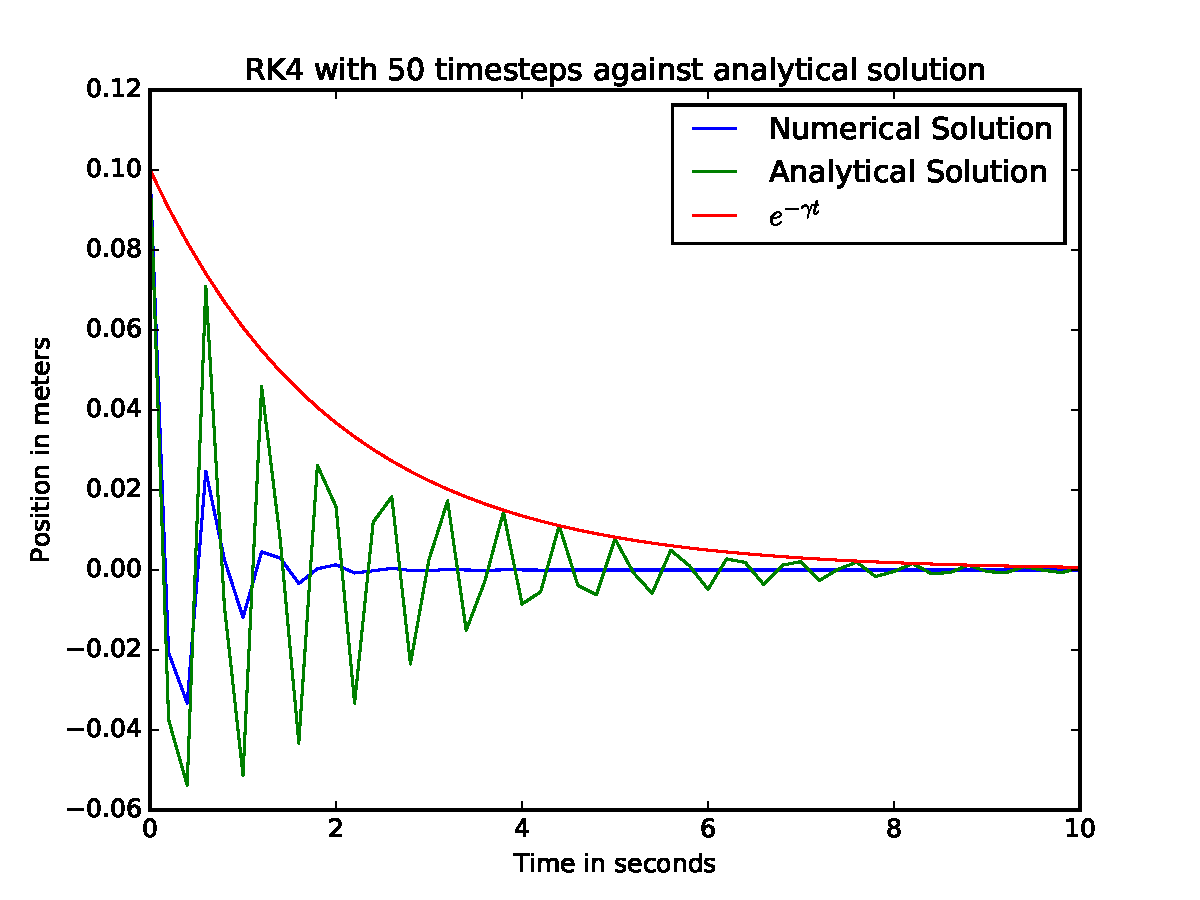
\includegraphics[width=0.5\textwidth]{fig/Pendulum50.pdf}
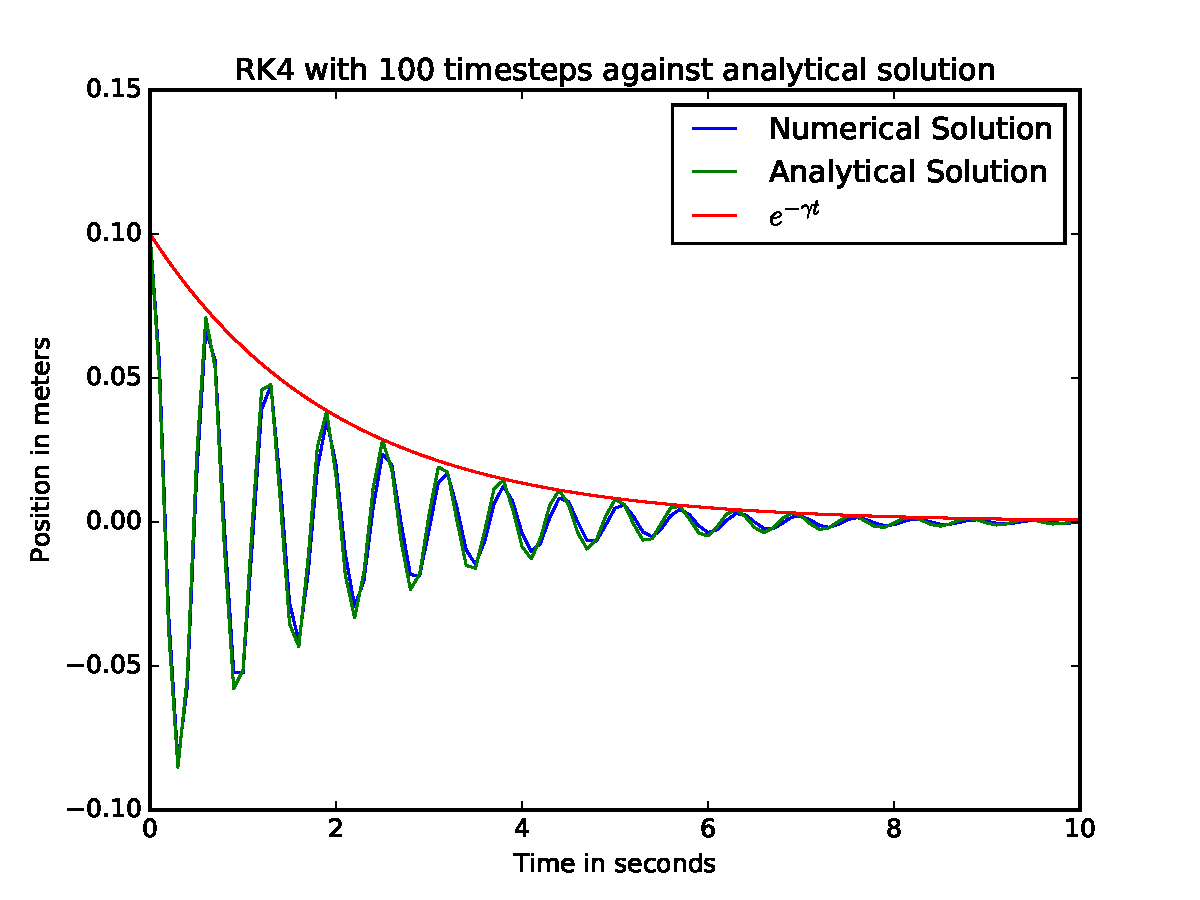
\includegraphics[width=0.5\textwidth]{fig/Pendulum100.pdf}
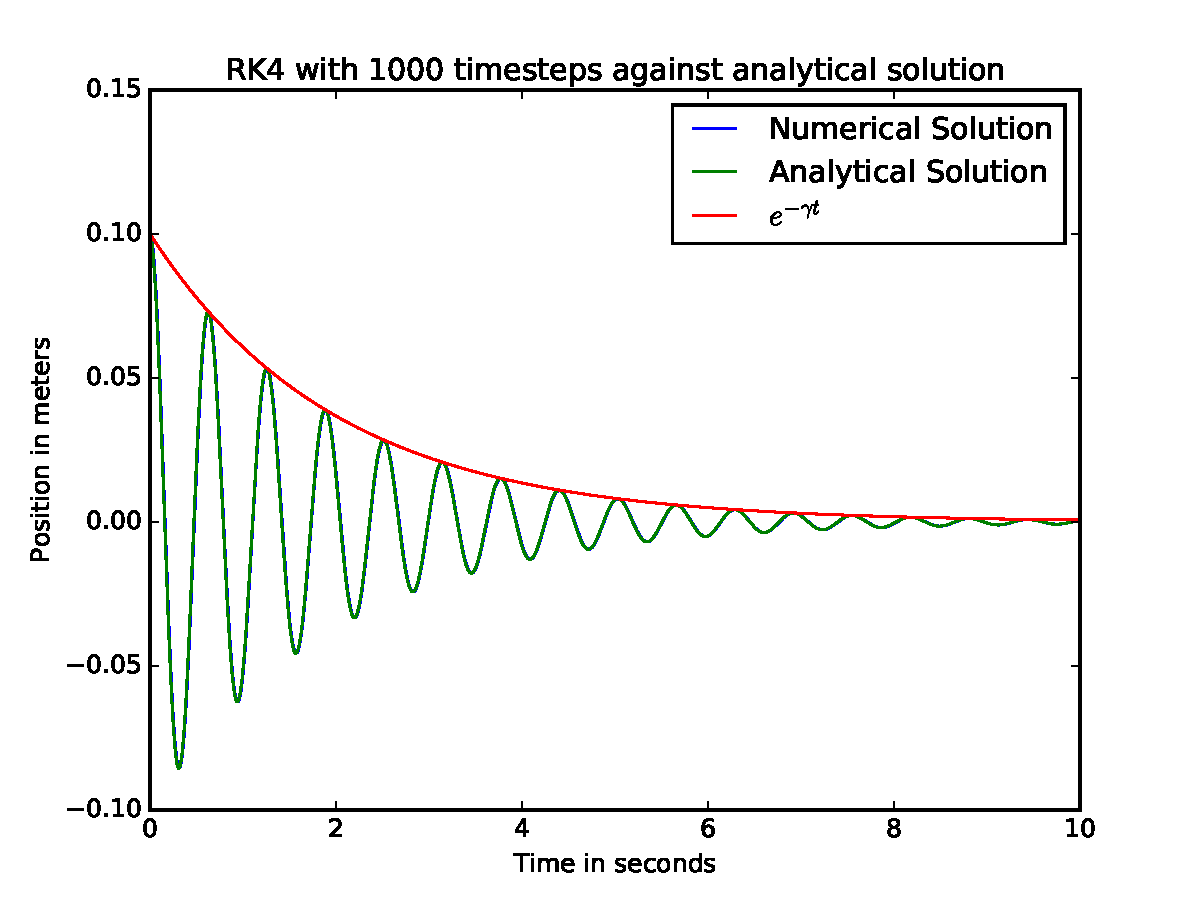
\includegraphics[width=0.5\textwidth]{fig/Pendulum1000.pdf}
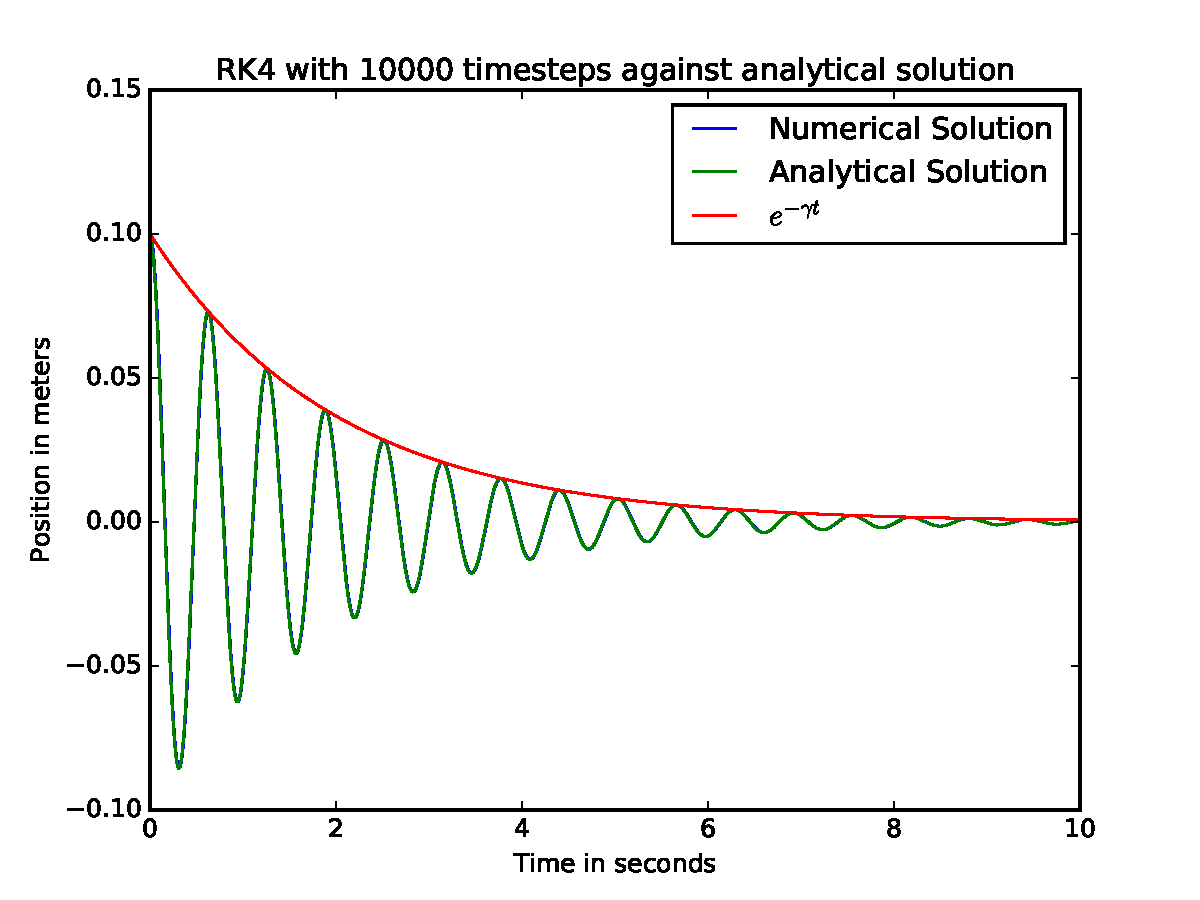
\includegraphics[width=0.5\textwidth]{fig/Pendulum10000.pdf}
\caption{Comparing analytical solution to numerical solution of RK4 over 10 seconds with 50, 100, 1000, and 10000 steps}
\label{fig:error}
\end{figure}

\begin{lstlisting}[basicstyle=\footnotesize,
frame = single,
label = lst:error,
caption = Error for different amount of steps of RK4]
Average error for 50 steps = 0.219415 cm
Largest error for 50 steps = 3.992651 cm
Average error for 100 steps = 0.032975 cm
Largest error for 100 steps = 0.745630 cm
Average error for 1000 steps = 0.003536 cm
Largest error for 1000 steps = 0.463238 cm
Average error for 10000 steps = 0.001118 cm
Largest error for 10000 steps = 0.463344 cm
Average error for 100000 steps = 0.000354 cm
Largest error for 100000 steps = 0.463346 cm
Average error for 1000000 steps = 0.000112 cm
Largest error for 1000000 steps = 0.463346 cm
\end{lstlisting}



\subsection*{b)}
Figur \ref{fig:dempning} viser de tre typene dempning av vårt svingningssystem. Ettersom kritisk dempning foregår ved $\omega = \gamma$, kan vi løse denne for $b$:
\begin{align*}
\omega &= \gamma \\
\sqrt{\frac{k}{m}} &= \frac{b}{2m} \\
b_{critical} &= \sqrt{4km}
\end{align*}
Heretter kan vi definere
\begin{align*}
b_{overcritical} &= b_{critical} + c \\
b_{undercritical} &= b_{critical} - d
\end{align*}
for to valgte positive tall $c$ og $d$. For å få en fin graf må disse må finnes gjennom prøving og feiling, men alle positive tall vil i prinsippet gi over- og under-dempning. Jeg valgte $c = 10$ og $d = 0.7$
\begin{figure}[H]
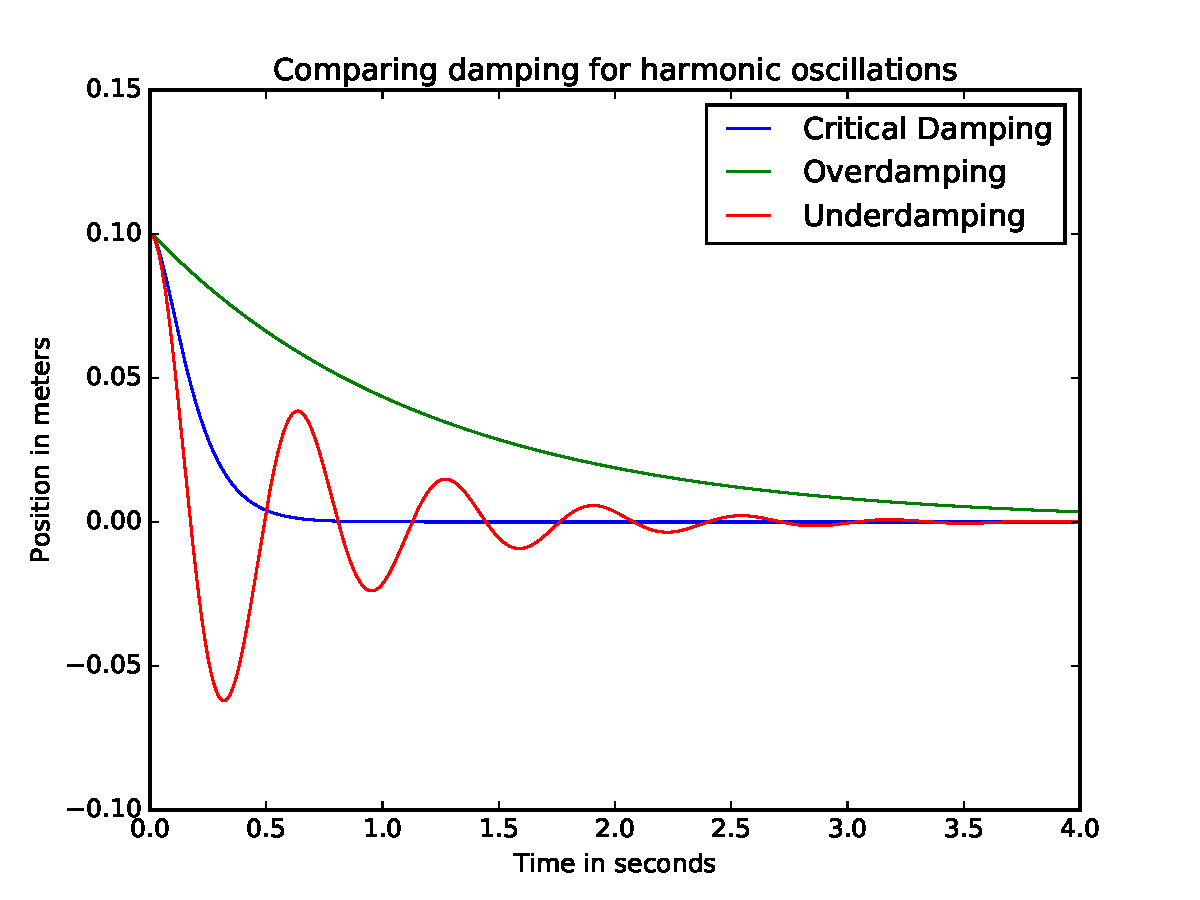
\includegraphics[width=\textwidth]{fig/Damping.pdf}
\caption{Visualisering av de tre typene dempning}
\label{fig:dempning}
\end{figure}



\subsection*{c)}
Vi har nå lagt til en påtrykt frekvens i programmet vårt, som kuttes av ved $t = 20\mathrm{s}$. I figur \ref{fig:resonans} ser vi hvordan utslaget av pendelen utvikler seg med en slik påtrykt kraft. I det første plottet er frekvensen til den påtrykte kraften lik egenfrekvensen til systemet, mens den i den andre grafen er satt til $0.9$ av egenfrekvensen.
\begin{figure}[H]
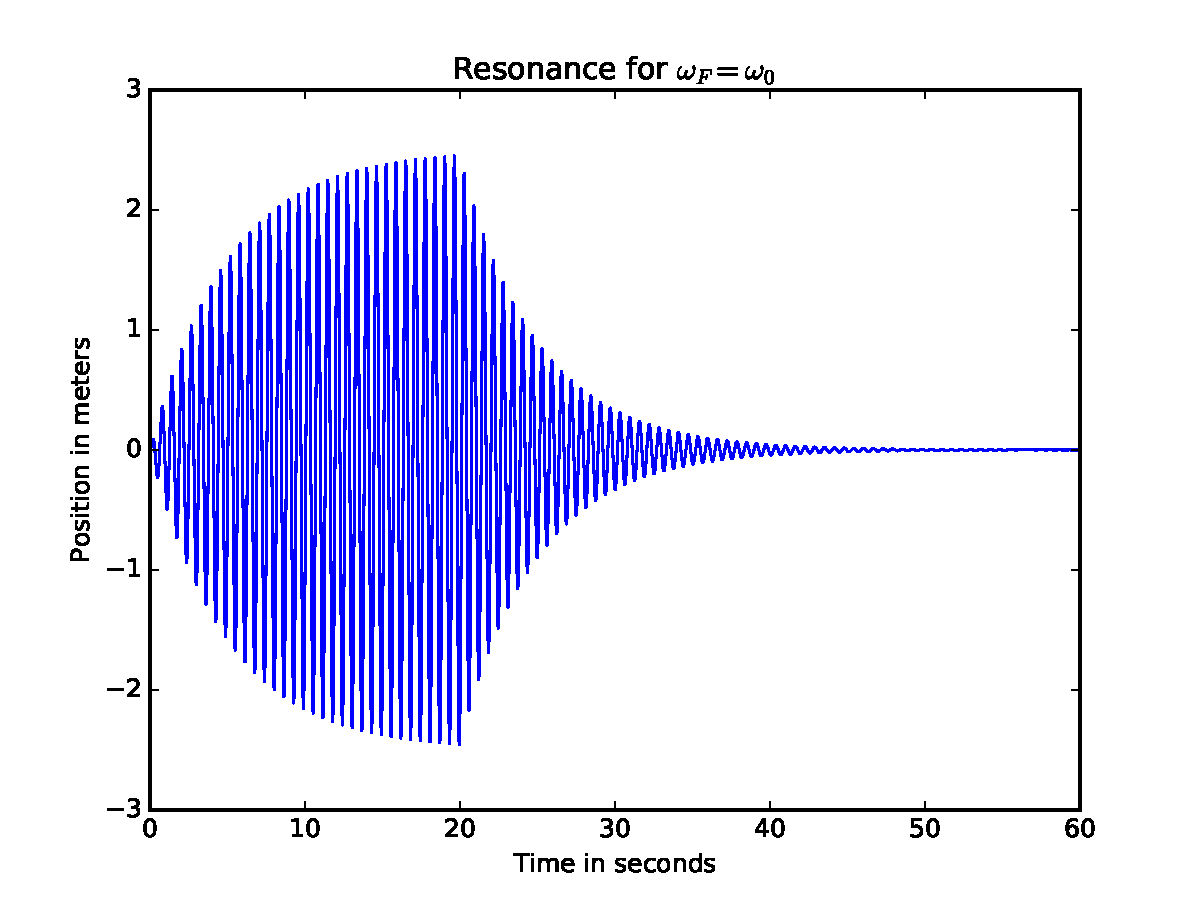
\includegraphics[width=0.5\textwidth]{fig/ResonanceSynced.pdf}
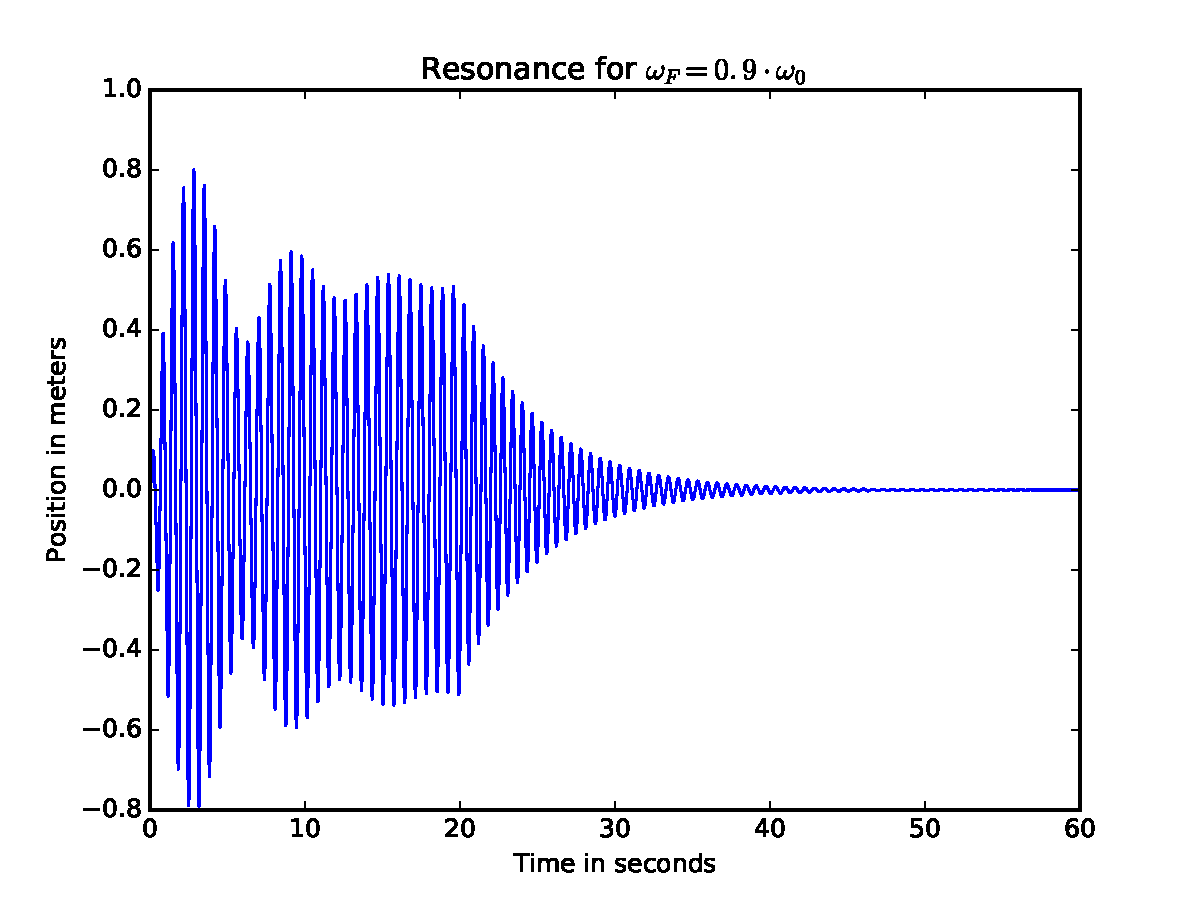
\includegraphics[width=0.5\textwidth]{fig/ResonanceUnsynced.pdf}
\caption{Sammenligning av påtrykt resonans med synkronisert og usynkronisert frekvens}
\label{fig:resonans}
\end{figure}



\subsection*{d)}
Nå må vi få programmet vårt til å kjøre over mange forskjellige simuleringer av påtrykte krefter med forskjellig frekvens. Jeg har valgt å variere denne frekvensen i intervallet $\omega_F \in [0, \ 2\omega_0]$, der $\omega_0$ er egenfrekvensen til systemet.\footnote{Jeg har laget en gif av hvordan svingningene utvikler seg ved forskjellige $\omega_F$ i dette intervallet. Den kan finnes på \href{https://www.dropbox.com/s/dwi7ei6tii6a9q9/Frequencies.gif?dl=0}{dennne} dropbox-linken. NB; Den er på 70MB.} Deretter må vi regne energien til hvert av systemene, og plotte energien mot frekvensen. Fra figur \ref{fig:freq} ser vi at plottet ser vi at plottet ligner det tilsvarende fra læreboken. Dersom vi leser av $\Delta f \approx 0.04$ fra figur \ref{fig:freq}, benytter oss av den eksperimentelle definisjonen av $Q$ fra læreboken, har vi at
\begin{align*}
Q = \frac{f_0}{\Delta f} \approx \frac{f_0}{0.04f_0} = 25
\end{align*}
 
\begin{figure}[H]
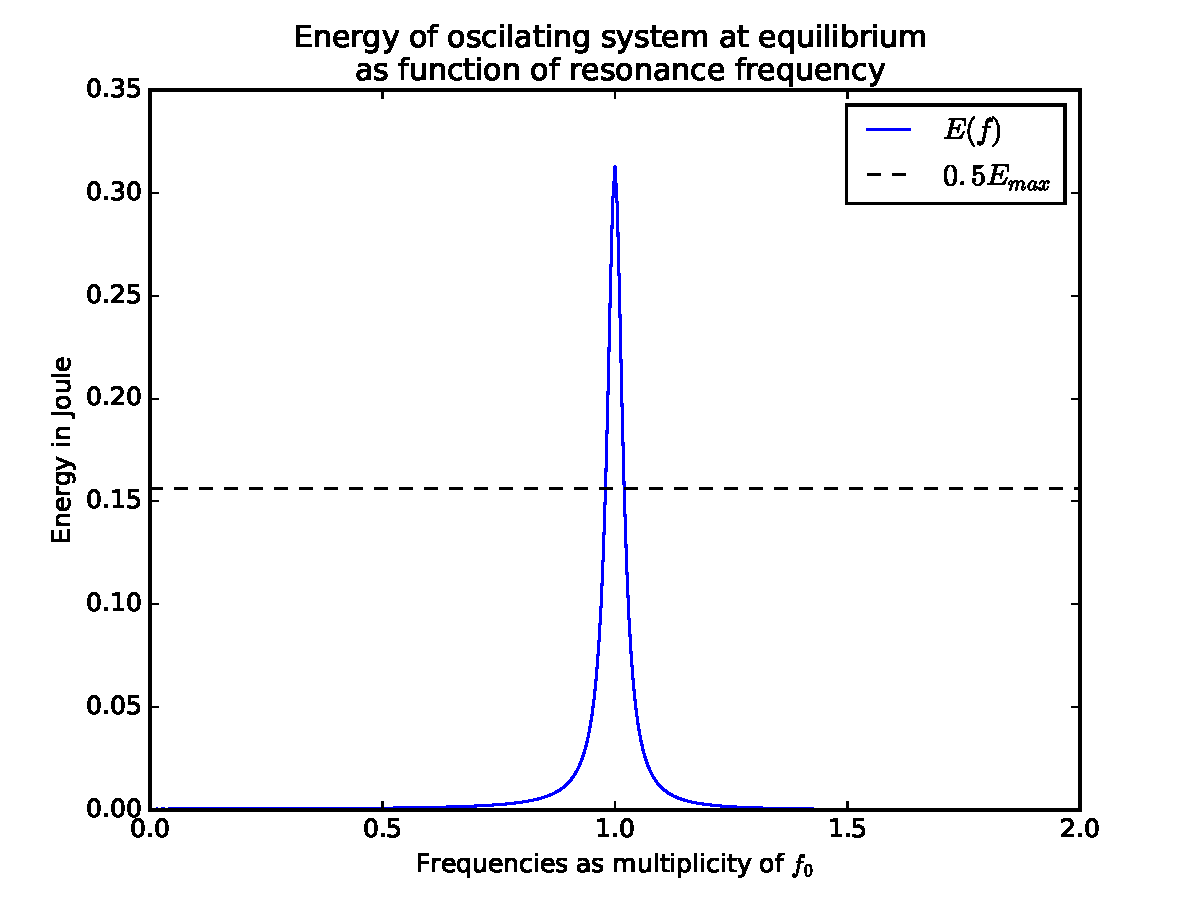
\includegraphics[width=0.5\textwidth]{fig/Frequency.pdf}
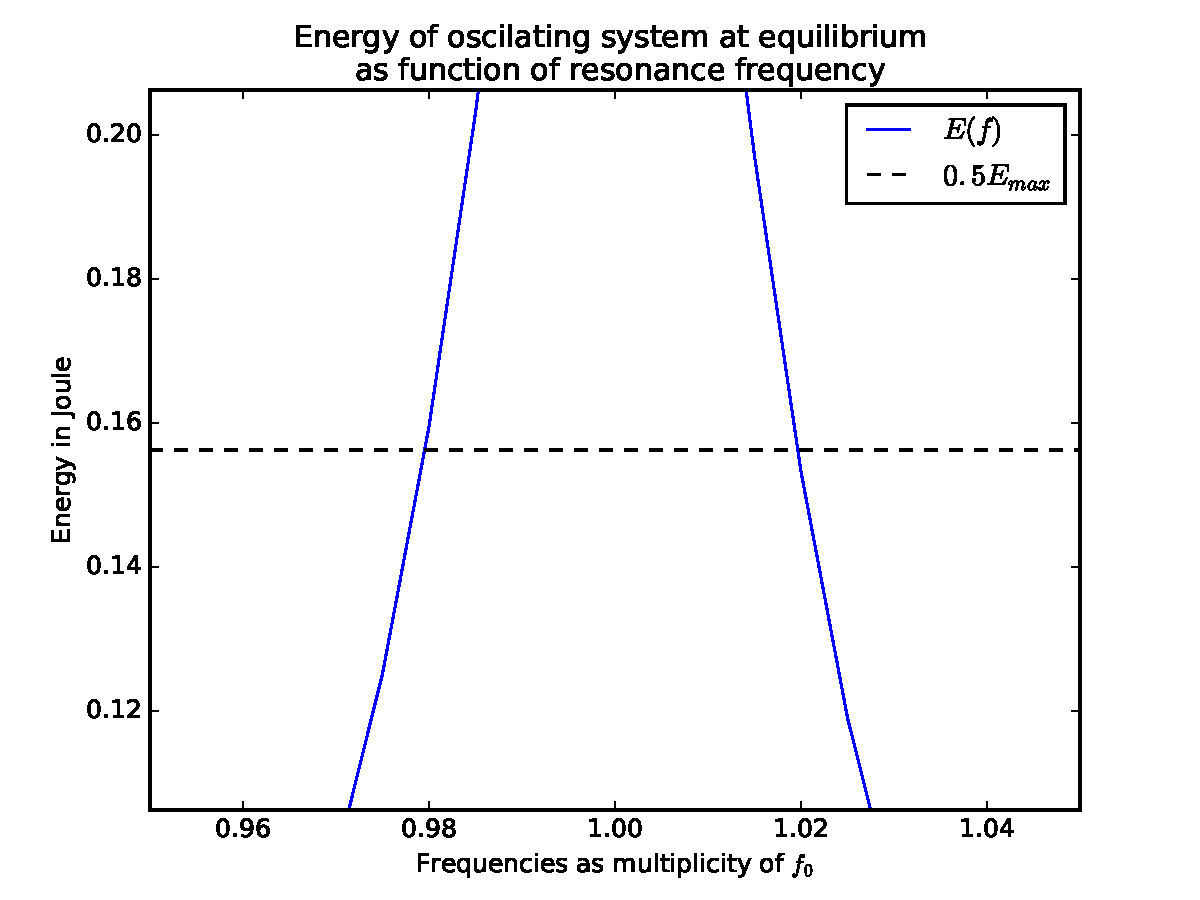
\includegraphics[width=0.5\textwidth]{fig/Frequency2.pdf}
\caption{Energi til system med resonans, som funksjon av frekvensen til den påtrykte kraften. Utsnitt av grafen til høyre.}
\label{fig:freq}
\end{figure}



\section*{Oppgave 7}
Vi har allerede studert frekvensresponsen til vårt system i forrige oppgave. Det gjenstår derfor bare å sammenligne dette med et analytisk uttrykk.

Hvis vi bruker den analytiske definisjonen av Q fra læreboken, har vi at
\begin{align*}
Q = \sqrt{\frac{mk}{b^2}} = \sqrt{\frac{0.1\mathrm{kg}\cdot 10\mathrm{kg/s^2}}{0.04^2\mathrm{kg^2/s^2}}} = \frac{1}{0.04} = 25
\end{align*}

Vi kan altså være meget fornøyde med vår numeriske tilnærming av $Q$ fra forrige oppgave.



\section*{Appendiks}
Dette appendikset inneholder et uløst mysterium. Dersom vi tar en titt på liste \ref{lst:error}, ser vi at ved 1000 tidssteg slutter den maksimale feilen å konvergere videre. Dersom vi tar en titt på figurene \ref{fig:mysterium} og \ref{fig:mysterium2}, ser vi at det helt fra starten forekommer en forskyvning av vår numeriske løsning. Det viser seg at samme hvor mye vi øker tidssteget så konvergerer ikke vår numeriske løsning på vår analytiske løsning, men derimot litt ved siden av. Denne forskyvningen forblir konstant gjennom hele simuleringen, og det er ikke snakk om en presisjonsfeil. Det kan heller ikke være snakk om en faktisk forskyvning i from av en $\phi$ i en løsning $A\cos(\omega t + \phi)$, fordi vi vet at pendelet begynner i sitt maksimale utslag, med 0 hastighet, og $\phi = 0$. Hvorfor denne forskyvningen oppstår forblir derfor et mysterium.

\begin{figure}[H]
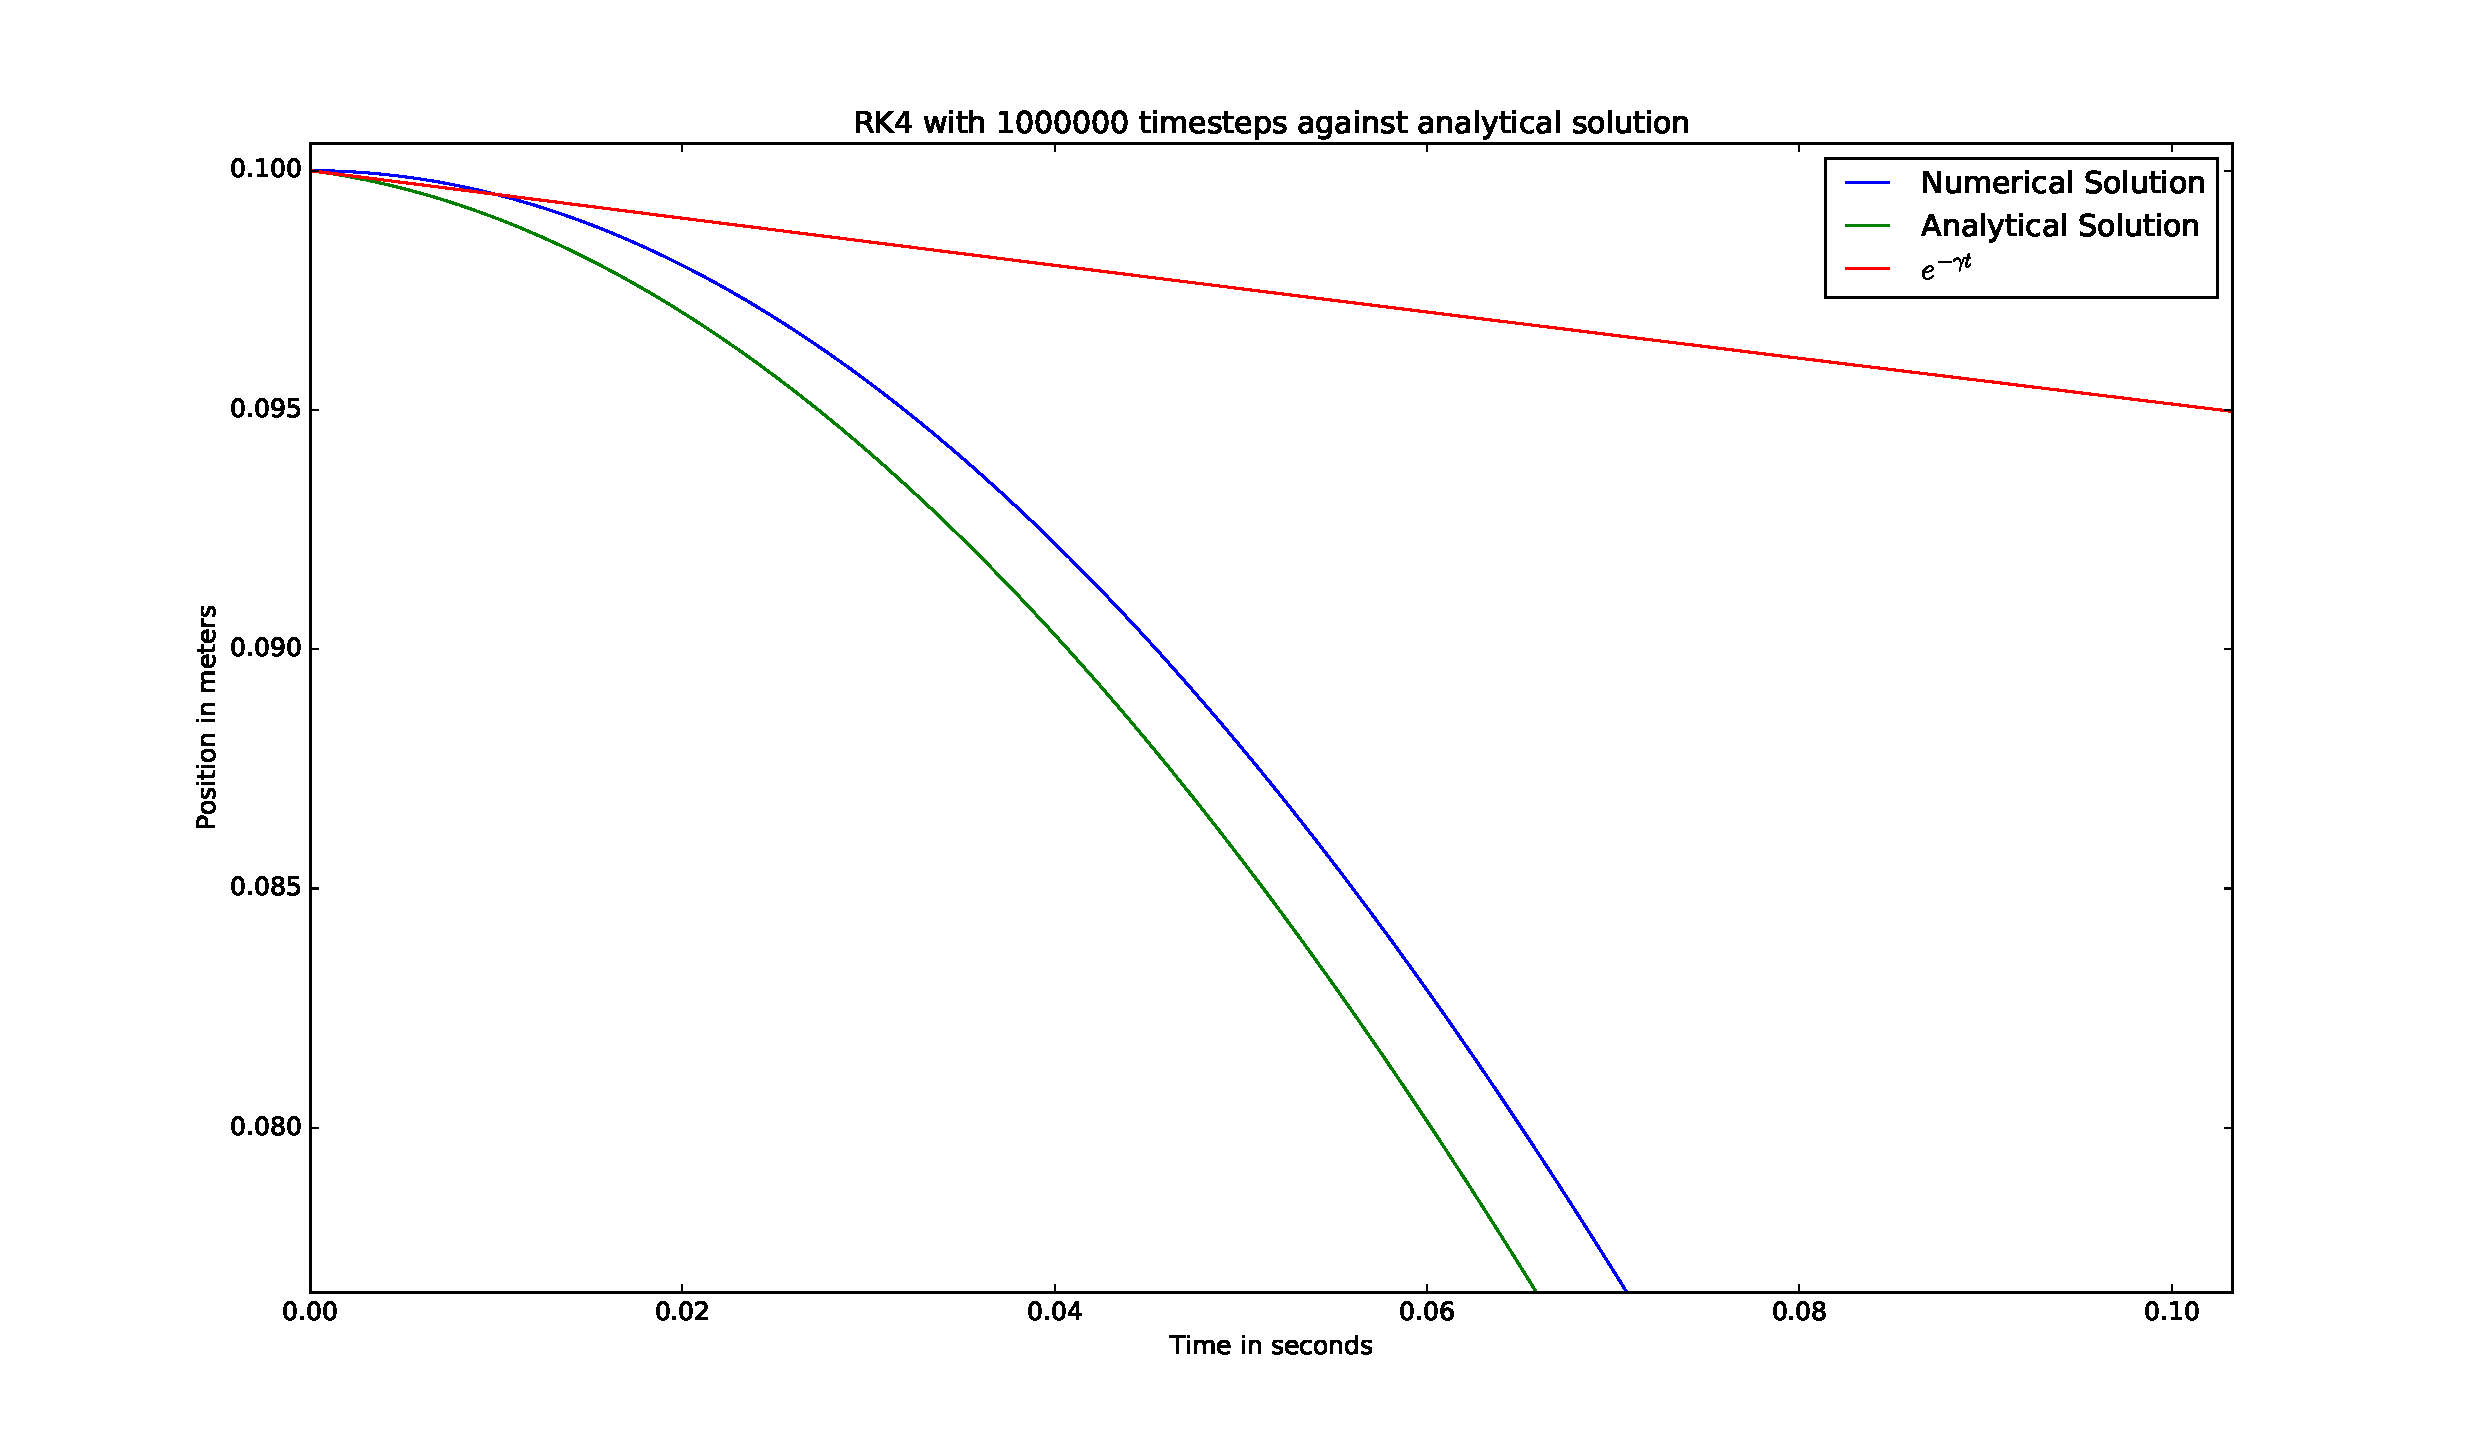
\includegraphics[width=\textwidth]{fig/Mysterium.pdf}
\caption{Forskyvning av numerisk løsning, av ukjente årsaker.}
\label{fig:mysterium}
\end{figure}

\begin{figure}[H]
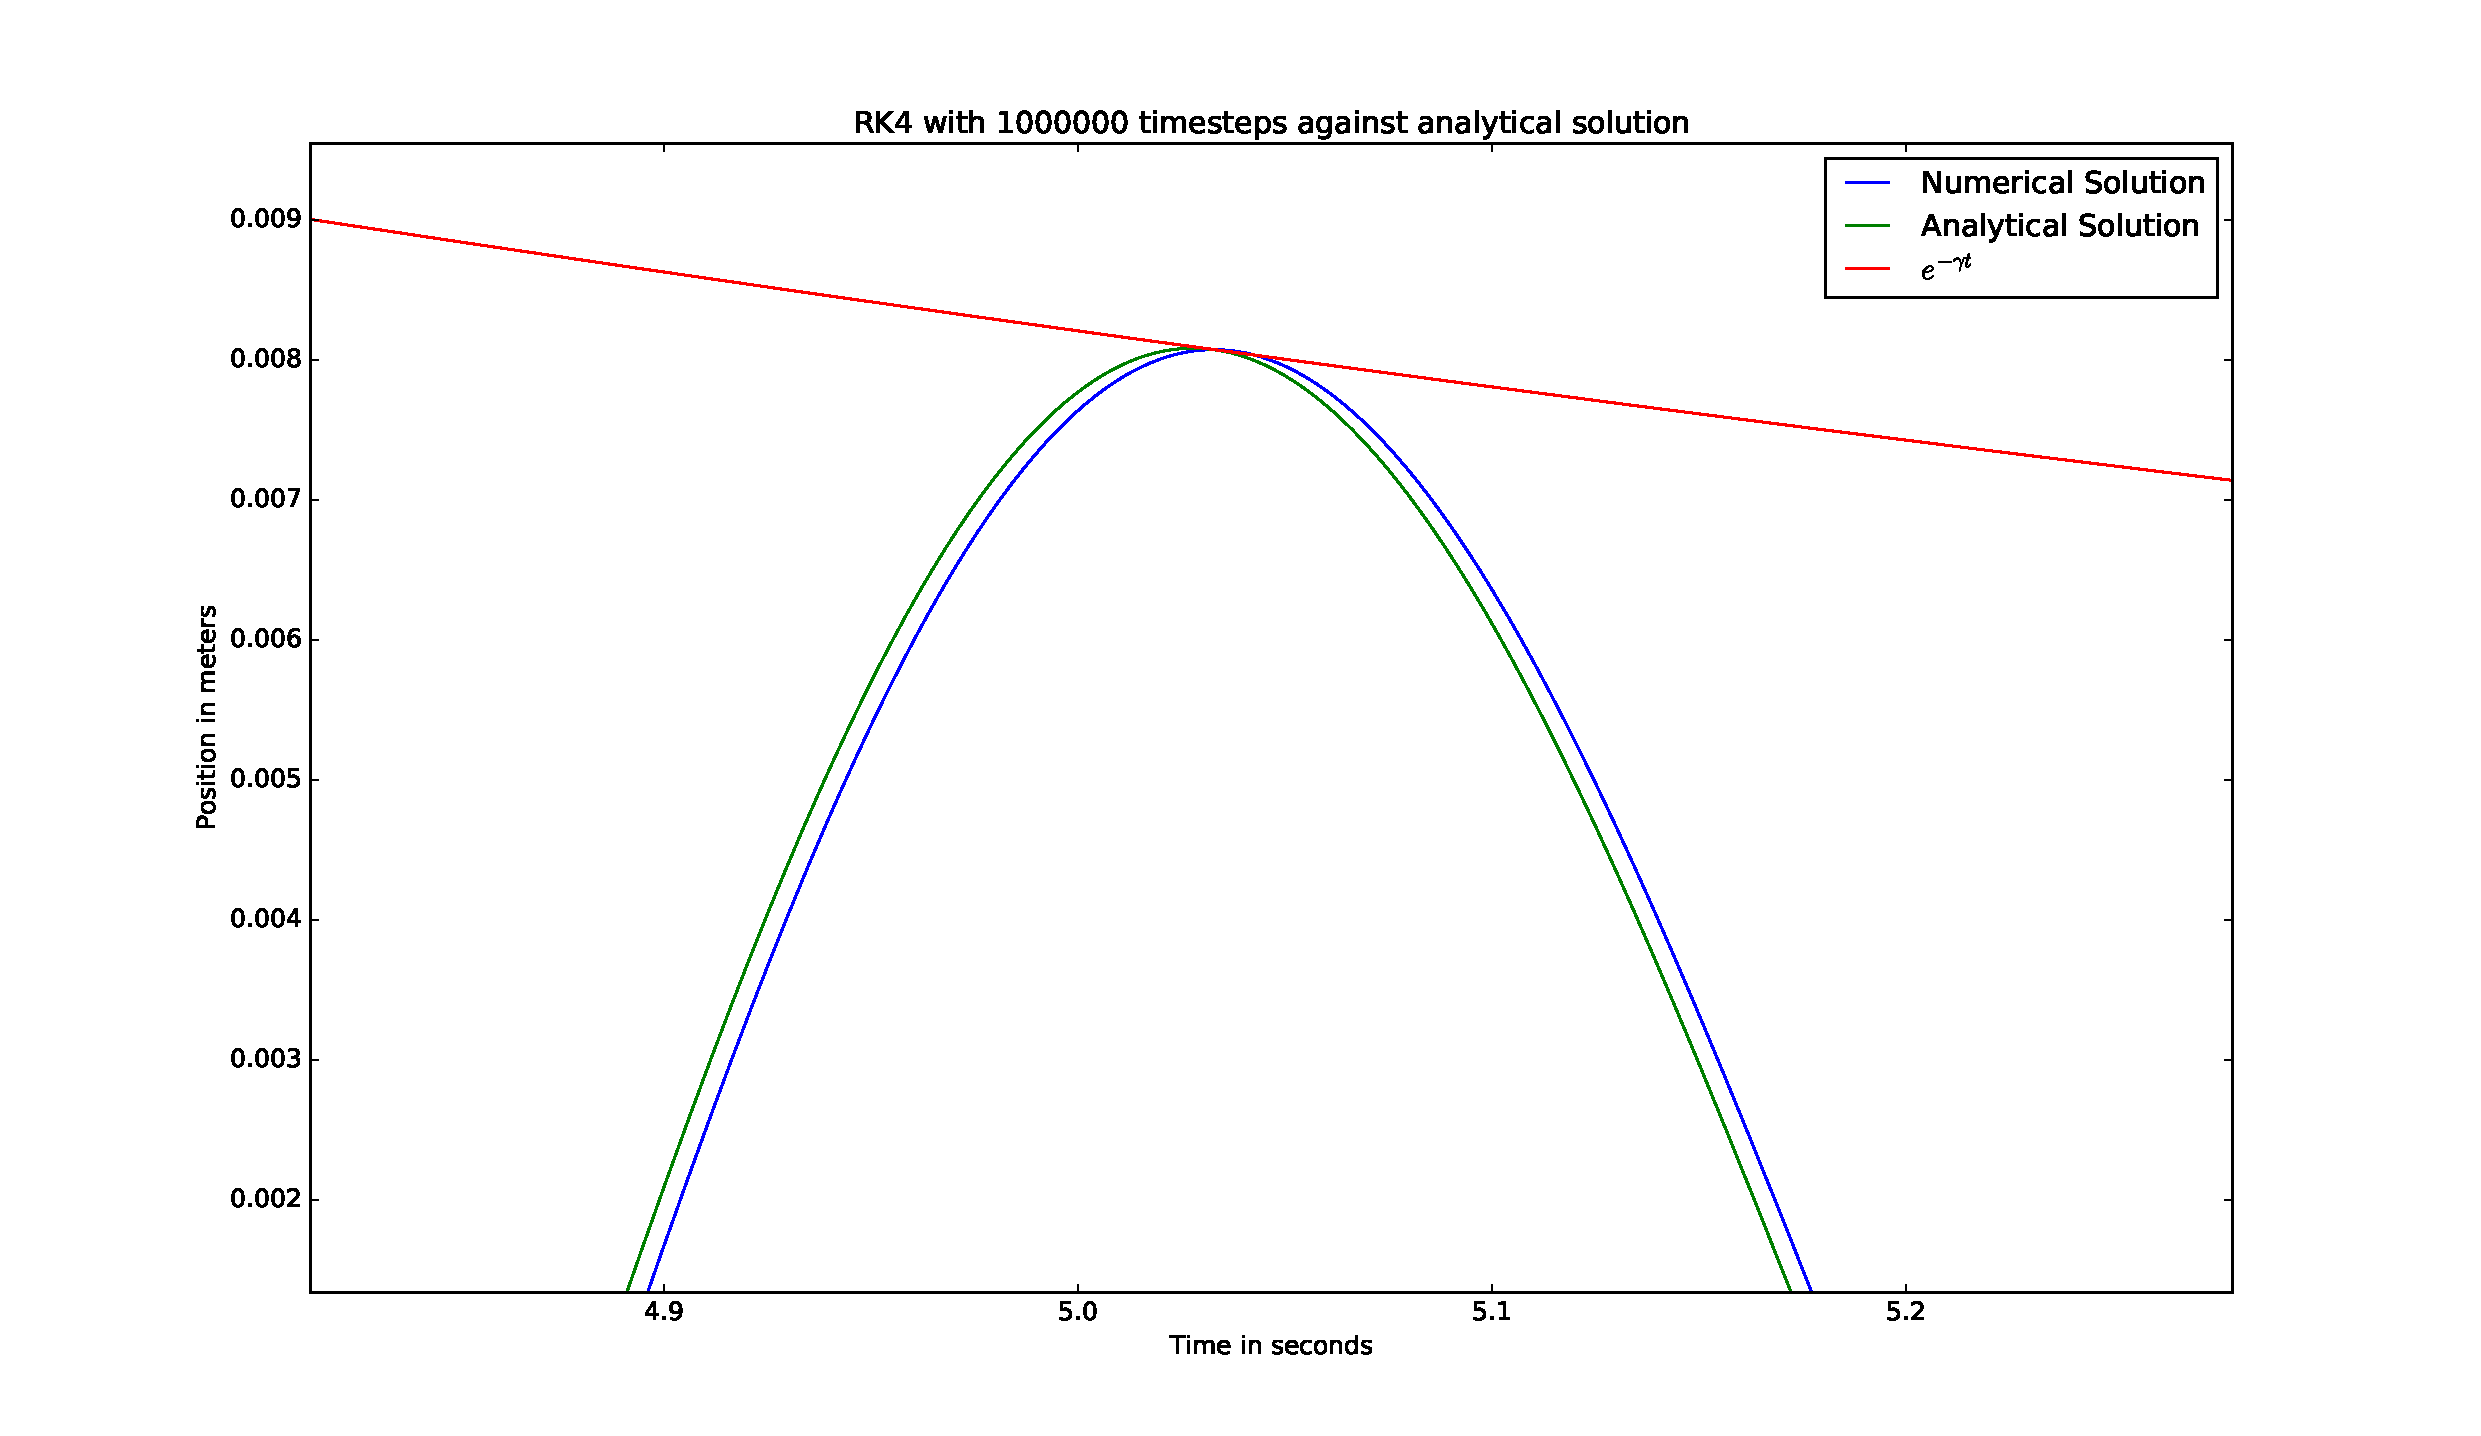
\includegraphics[width=\textwidth]{fig/Mysterium2.pdf}
\caption{Forskyvning av numerisk løsning, av ukjente årsaker.}
\label{fig:mysterium2}
\end{figure}

\end{document}
